\documentclass{officialexam} 
\usepackage{circuitikz}
%\everymath{\color{blue}}
\usepackage{graphicx}
\graphicspath{ {./images/} }
\begin{document}
	\begin{center}
		\kml ប្រឡងឆមាសលើកទី២\\
		វិញ្ញាសា: រូបវិទ្យា(ថ្នាក់ទី១១)\\
		រយៈពេល: ៩០ នាទី\\
		ពិន្ទុសរុប: ៧៥ ពិន្ទុ
	\end{center}
	\begin{center}
		\underline{\kml \color{blue}ប្រធាន:}
	\end{center}
	\begin{enumerate}[I]
		\item (១០ ពិន្ទុ) ចល័តមួយបានផ្លាស់ទីពីទីតាំងទី១ $x_1=\left(3+6t\right)m$ និង $y_1=\left(-5+3t\right)m$ ទៅទីតាំងទី២ $x_2=\left(5+6t\right)m$ និង $y_2=\left(-5-3t\right)m$។
		គណនាបម្លាស់ទីនៃចល័តនោះនៅខណៈ $t=1s$។
		\item (១០ ពិន្ទុ) គណនាមាឌឧស្ម័ននីត្រូសែន $2.8g$ ដែលផ្ទុកក្នុងធុងក្រោមសម្ពាធ $2.0\times10^{5}Pa$ និងសីតុណ្ហភាព $127^\circ C$ ។ \\គេឲ្យ $R=8.31J/mol\cdot K$ និងម៉ាសម៉ូលេគុលឧស្ម័ននីត្រូសែន $M(N_2)=28g/mol$
		\item (១០ ពិន្ទុ) ប្រភពលំញ័រនៃខ្សែតូចឆ្មាមួយមានសមីការចលនា $y=6\sin\left(100\pi t+ \frac{\pi}{4}\right)$ ដែល $y$ គិតជា $cm$ និង $t$ គិតជា $s$។\\ ប្រភពនេះបញ្ចូនរលកដាលផុតខ្សែប្រវែង $12.0m$ ក្នុងរយៈពេល $3.0s$។
		\begin{enumerate}[k]
			\item គណនាល្បឿនដំណាលរលកនៃលំញ័រនេះ។
			\item គណនាអំព្លីទុត មុំផាសដើម ខួប ប្រេកង់ និងជំហានរលកនៃលំញ័រនេះ។
		\end{enumerate}
		\item (១៥ ពិន្ទុ) ភាគល្អិតមួយមានវិុចទ័រទីតាំងកំណត់ដោយ $\vec{r}=\left(4\cos t\vec{i}+4\sin t\vec{j}\right)m$ ។
		\begin{enumerate}[k]
			\item កំណត់វិុចទ័រល្បឿន និងវុិចទ័រសំទុះរបស់ភាគល្អិត។
			\item គណនាសំទុះរបស់ភាគល្អិត។
		\end{enumerate}
		\item (២០ ពិន្ទុ) វុិចទ័រទីតាំងនៃចំណុចរូបធាតុមួយកំណត់ដោយ $\vec{r}=3.00\vec{i}-6.00t^2\vec{j}$ ដែល $\vec{r}$ គិតជា $m$ និង $t$ គិតជា $s$។
		\begin{enumerate}[k]
			\item កំណត់វិុចទ័រល្បឿនជាអនុគមន៍នៃពេល។
			\item កំណត់វុិចទ័រសំទុះនៃចំណុចរូបធាតុជាអនុគមន៍ពេល។
			\item ចូរគណនាតម្លៃនៃវុិចទ័រទីតាំង និងវុិចទ័រល្បឿន នៅខណៈ $t=1.00s$។
		\end{enumerate}
		\item (១០ ពិន្ទុ) កូនបាល់មួយត្រូវបានទាត់ចេញពីចំណុច $A$ ដោយក្មេងប្រុសម្នាក់ មានល្បឿនដើម $\nu_A=10m/s$ បង្កើតបានមុំ\\ $30^\circ=\frac{\pi}{6}rad$ ជាមួយនឹងអ័ក្សដេកដូចបានបង្ហាញក្នុងរូប។
		\begin{multicols}{2}
			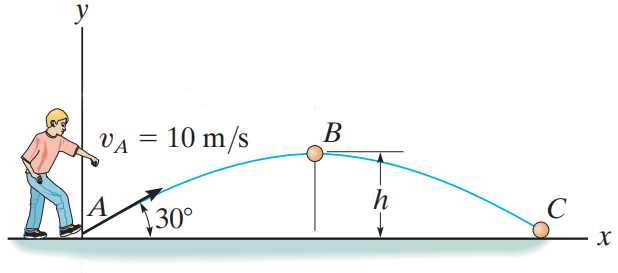
\includegraphics[scale=1.8, height=128pt]{pic2}
			\begin{enumerate}[k]
				\item ចូរសរសេរសមីការគន្លងនៃចលនារបស់គ្រាប់បាល់។
				\item ចូរគណនាចម្ងាយធ្លាក់ $x$ របស់គ្រាប់បាល់ពេលវាធ្លាក់ដល់ចំណុច $C$។\\
				គេឲ្យ $g=10m/s^2$ និង\\ $\cos\frac{\pi}{6}=\frac{\sqrt{3}}{2},~\sin\frac{\pi}{3}=\frac{\sqrt{3}}{2}, \tan\frac{\pi}{6}=\frac{\sqrt{3}}{3}$
			\end{enumerate}
		\end{multicols}
	\end{enumerate}
\end{document}